\appendix
\label{sec:appendix}

\chapter{Middleware Implementations}
\label{sec:apdx-middleware-implementations}

\lstinputlisting[language=Go, caption={Logging Middleware Implementation}]{code-snippets/logging-middleware.go.bak}

\lstinputlisting[language=Go, caption={Max Bytes Middleware Implementation}]{code-snippets/max-bytes-middleware.go.bak}

\chapter{Screenshots of Frontend Design}
\label{sec:apdx-screenshots}

\begin{figure}[htbp]
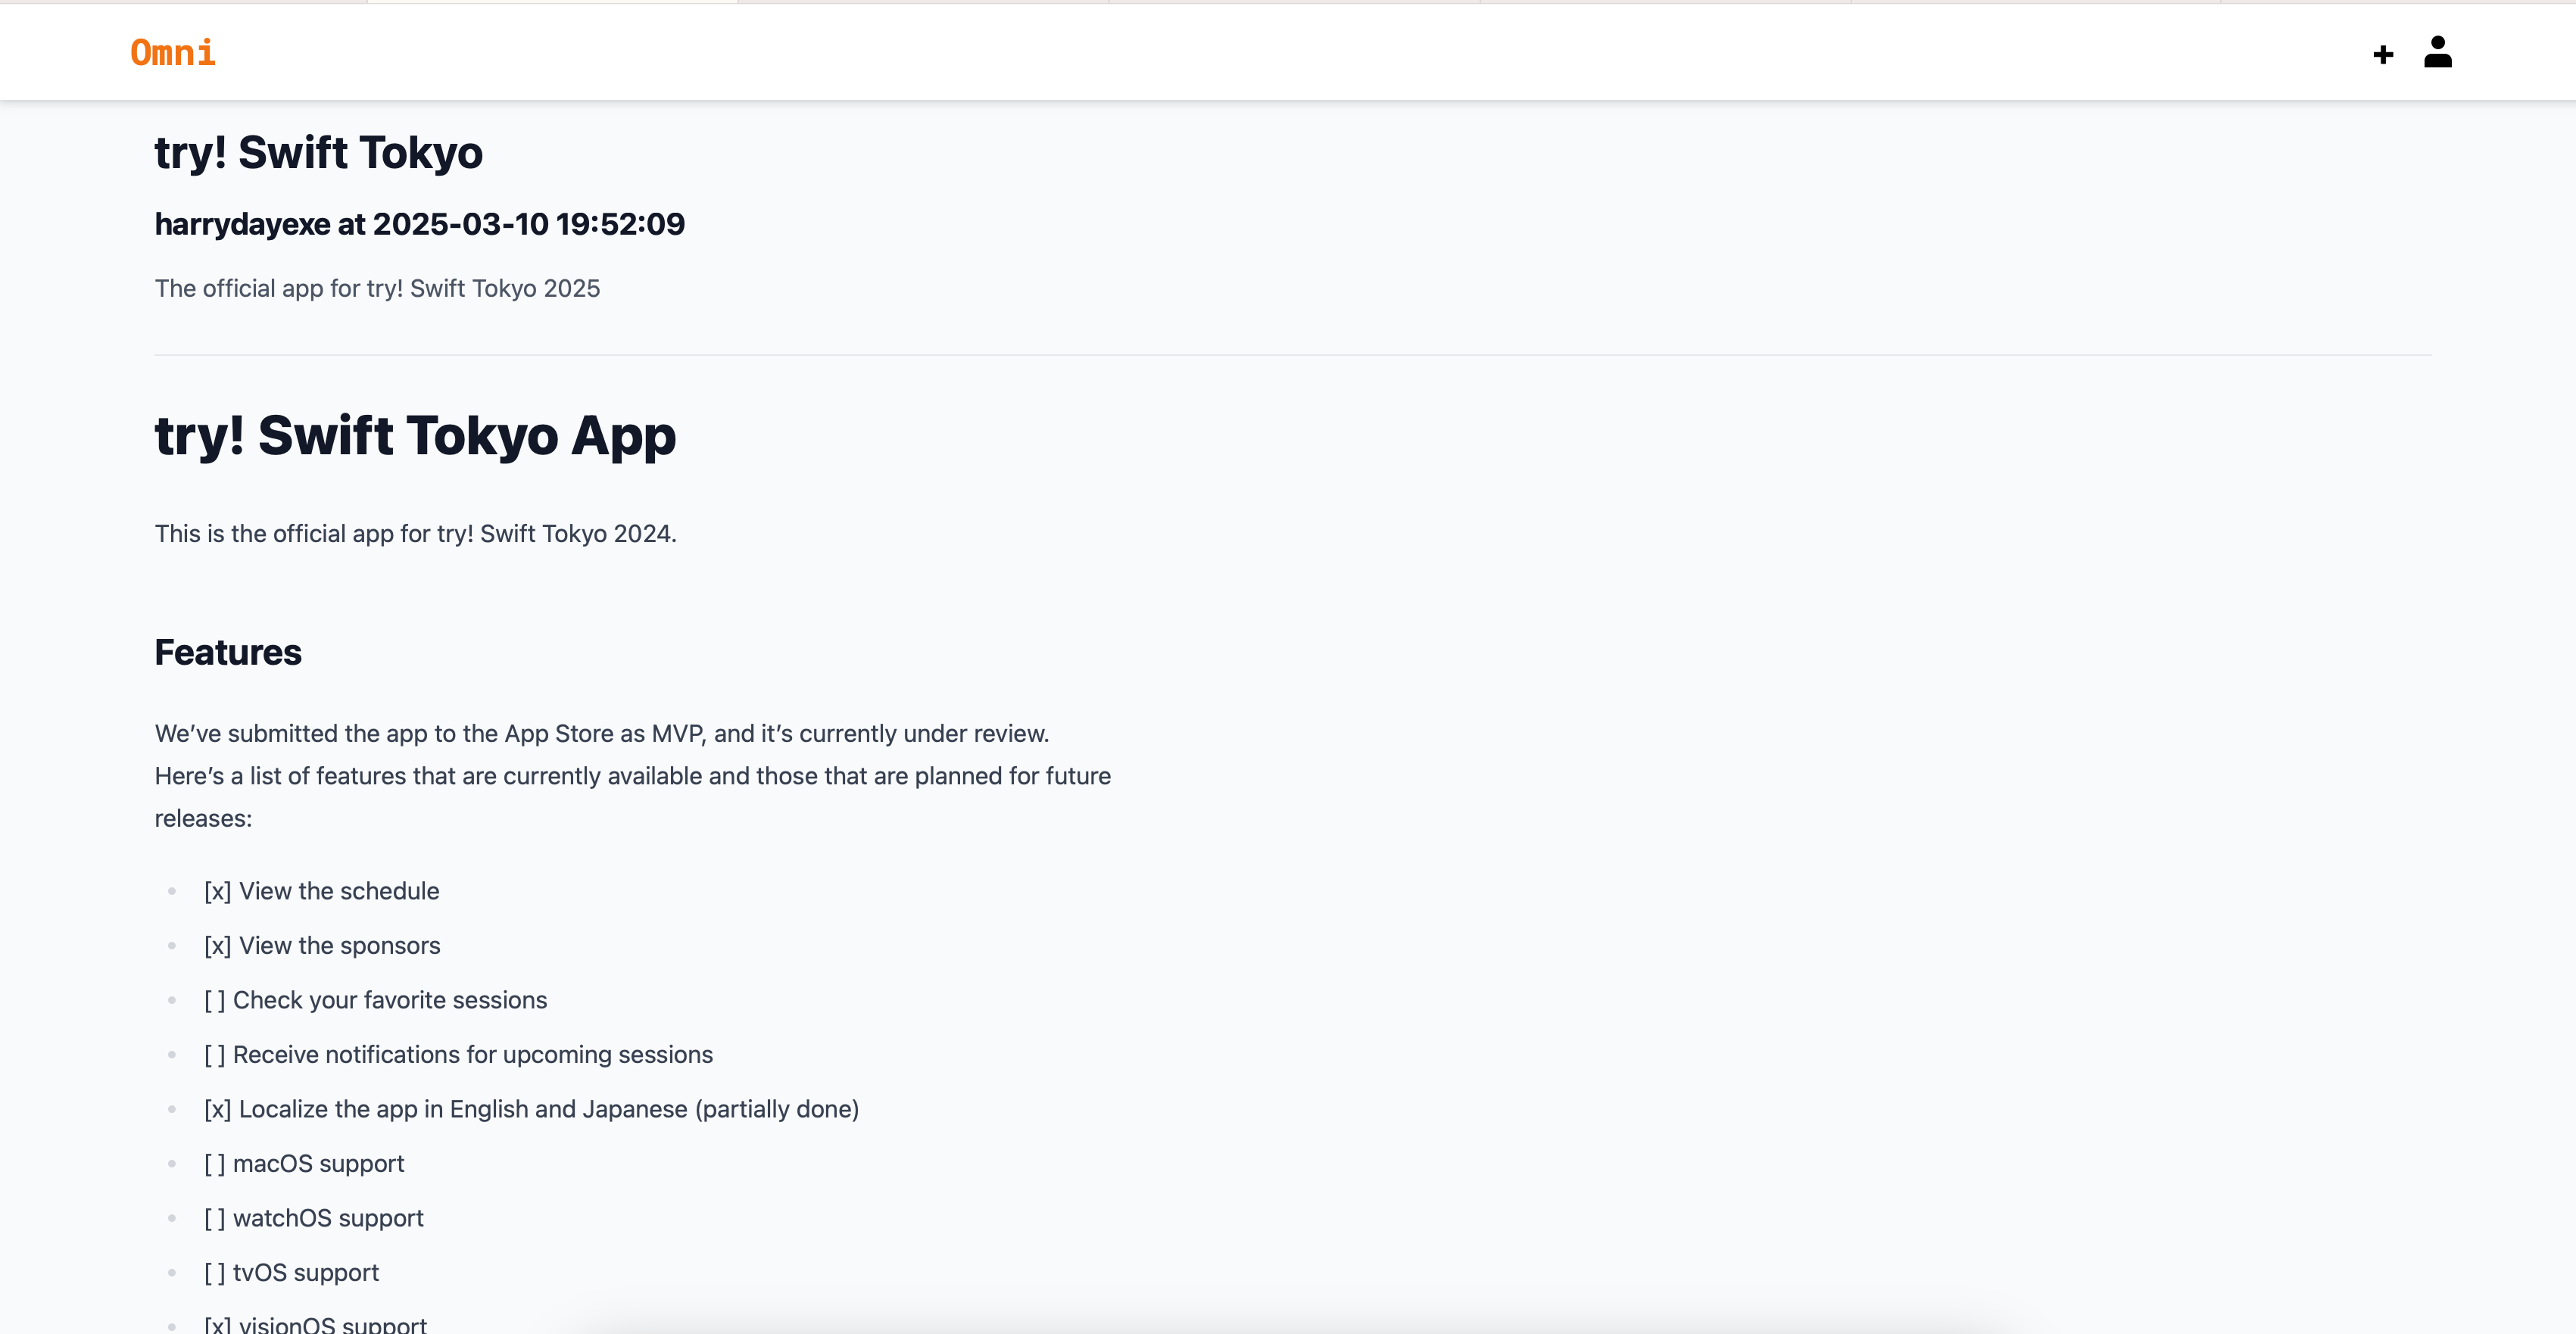
\includegraphics[width=12cm]{post-page-light.png}
\centering
\caption{Omni Post Page (Light Mode)}
\end{figure}

\begin{figure}[t]
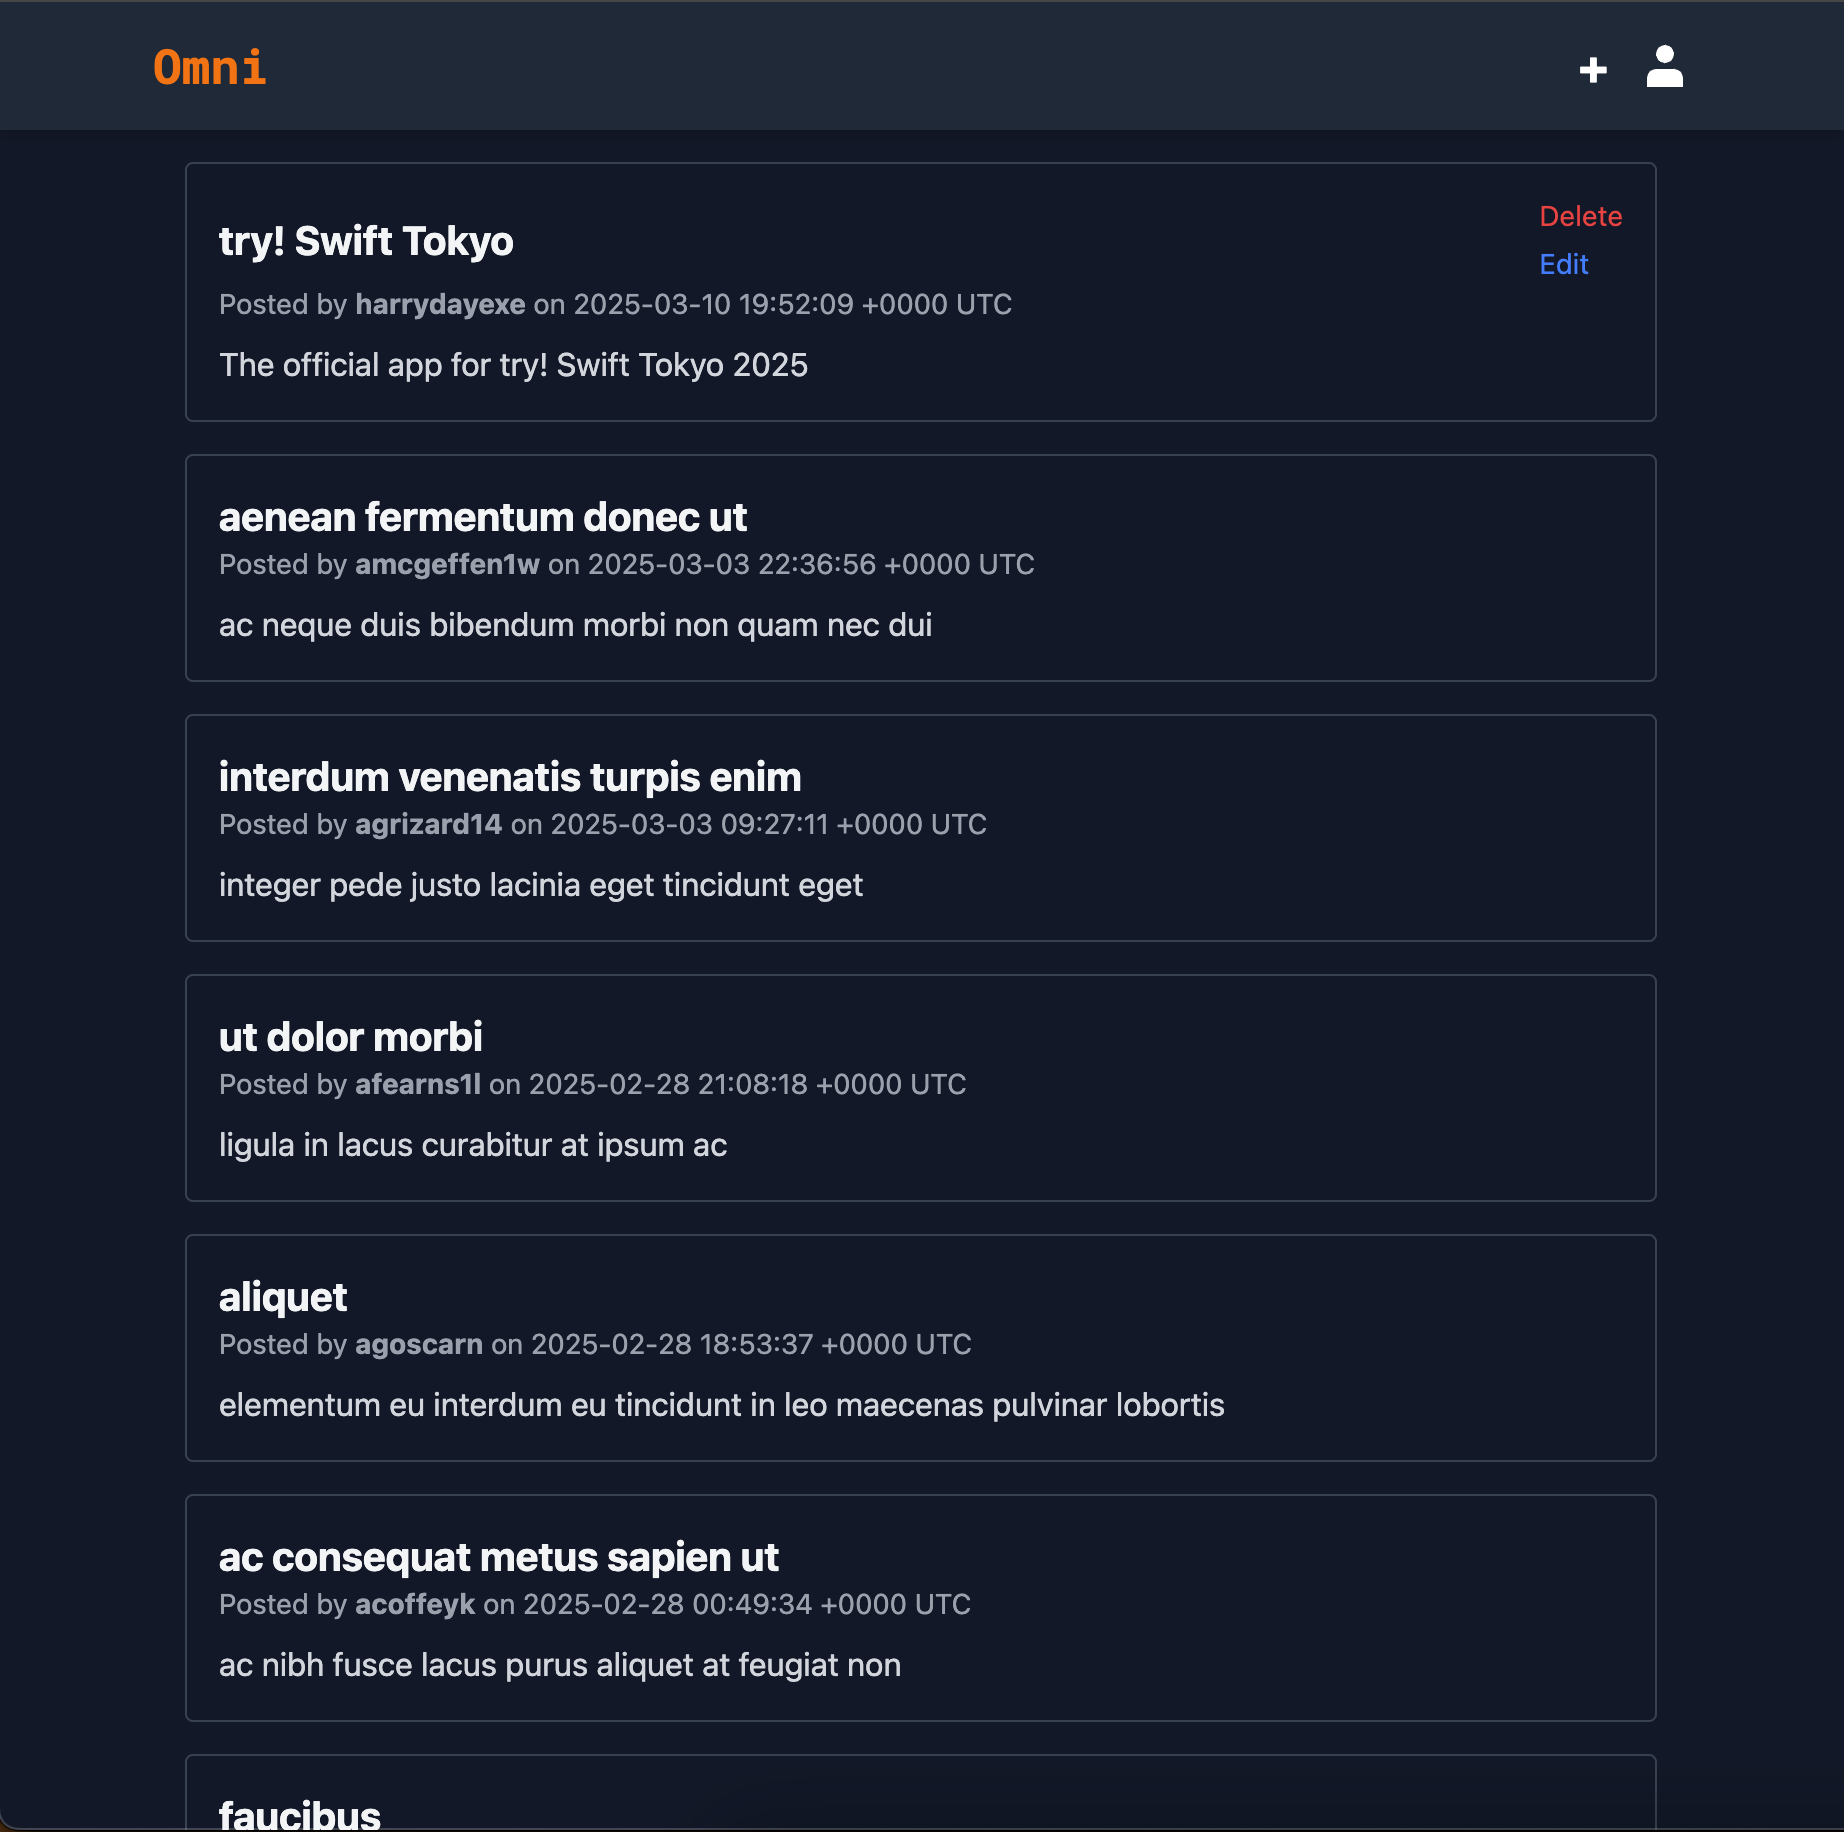
\includegraphics[height=9cm]{home-dark.png}
\centering
\caption{Omni Home Page (Dark Mode)}
\end{figure}

\begin{figure}[b]
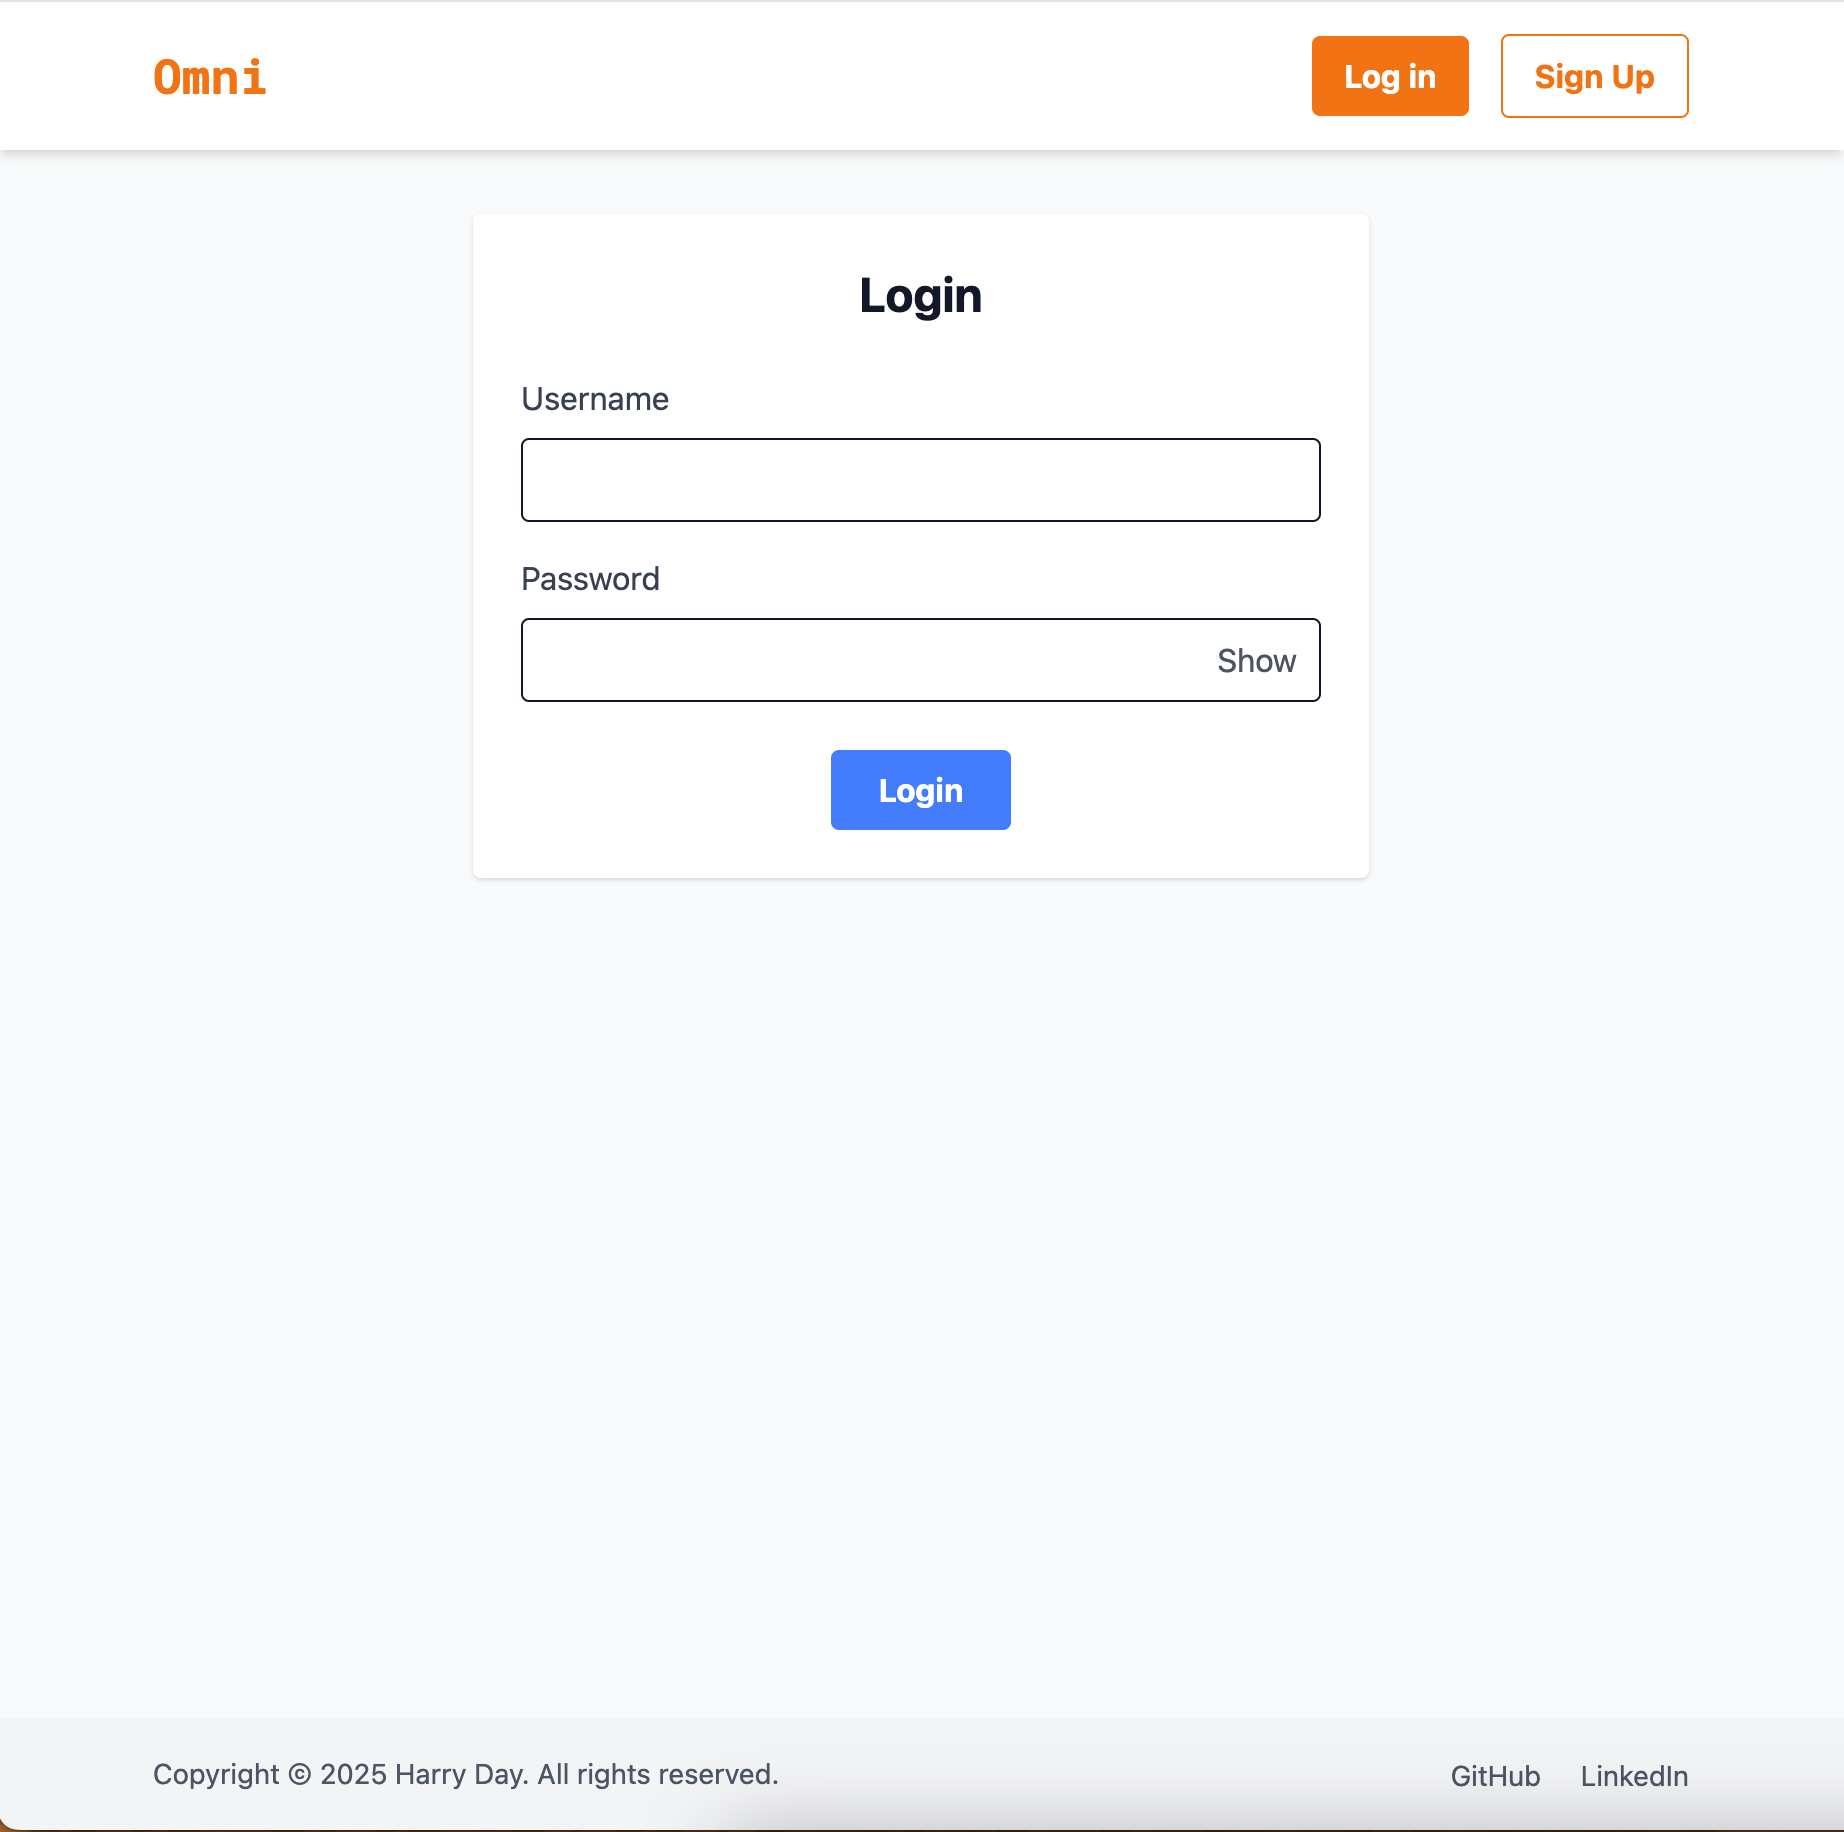
\includegraphics[height=9cm]{login-light.png}
\centering
\caption{Omni Login Page (Light Mode)}
\end{figure}

\begin{figure}[htbp]
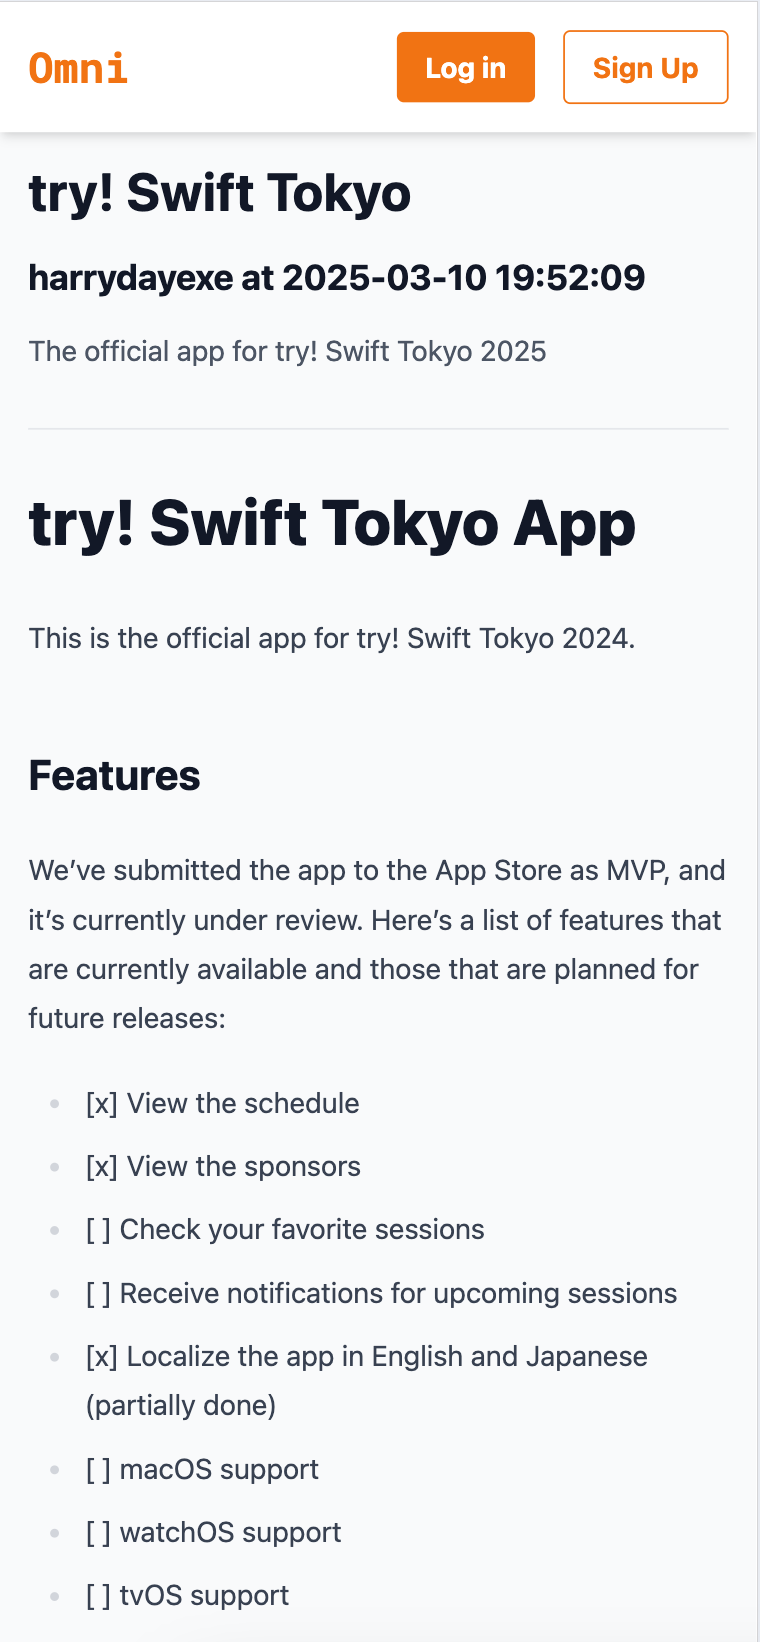
\includegraphics[height=12cm]{post-page-phone.png}
\centering
\caption{Omni Post Page (Mobile)}
\end{figure}

\chapter{Concurrency in OmniView}
\label{sec:apdx-concurrency-omni-view}

\lstinputlisting[language=Go, caption={Concurrency in OmniView}]{code-snippets/concurrency-support.go.bak}

\chapter{User Survey Responses}
\label{sec:apdx-user-survey}

\section{Questions}
\begin{itemize}
    \item How easy or difficult did you find the site to navigate? For example, when creating an account, viewing posts or writing a comment?
    \item Would the platform be helpful to you as a junior software engineer?
    \item Do you see yourself primarily producing or consuming content on Omni?
\end{itemize}

\section{Responses}

\subsection{Participant 1}
\subsubsection{Question 1}
Using Omni was a breeze! Everything went really well, from registering to responding to posts. I appreciated how easy the site was to navigate; I never got lost.

\subsubsection{Question 2}
Of course. It seems like a great place to learn and maintain ties with the tech community. It would be really beneficial for my development to have access to project ideas, industry discussions, and advice in one location.

\subsubsection{Question 3}
I would primarily be consuming content and learning at the moment. However, I'd love to eventually start sharing my own projects and advice as well.

\subsection{Participant 2}
\subsubsection{Question 1}
I found Omni to be very user-friendly. Whether I was reading posts or leaving comments, it was easy to find what I needed thanks to the simple design.

\subsubsection{Question 2}
Yes, absolutely! It appears to be a fantastic resource for both more complex subjects and advice aimed at beginners. I could see it greatly advancing my skill set.

\subsubsection{Question 3}
I'll primarily consume content to learn at first, but eventually I'd like to share interesting things I find or create tutorials.

\subsection{Participant 3}
\subsubsection{Question 1}
I had no trouble navigating Omni. The layout made it very easy to begin interacting, and creating an account was quick. It felt very natural to write comments and posts; the platform seems to be designed to make producing posts as simple as possible.

\subsubsection{Question 2}
Of course. Omni seems like the perfect platform for me to post tutorials, share my learning experiences, and even initiate conversations with other community members. Having a platform that makes contributing so easy and friendly is encouraging.

\subsubsection{Question 3}
Without a doubt, my primary goal is to produce content. I can't wait to share resources, write posts, and perhaps even document some of my ongoing projects. It seems like a wonderful place to learn and give back.

\subsection{Participant 4}
\subsubsection{Question 1}
The site follows the classic design conventions that social networks use, which assisted in finding the correct buttons and ui elements for creating an account and posting. 

\subsubsection{Question 2}
Yes, using the READMEs that I have already written for my projects is an innovative idea that reduces the barrier to producing content. It makes it very easy to share my projects quickly.

\subsubsection{Question 3}
I would primarily be producing content to help my CV, but I would also be consuming content to get ideas from others. I think it is a great idea to have a platform that allows you to do both.

